\chapter{\IfLanguageName{dutch}{Resultaten van de simulaties}{Results of the simulations}}
\label{ch:resultaten-simulaties}
In dit hoofdstuk worden de resultaten van de verschillende simulaties weergeven. De simulaties werden uitgevoerd met een zelf geschreven simulatietool waarvan de code zich in bijlage bevindt. Voor elke set van parameters in tabel \ref{tab:parameters} wordt er 30 keer een simulatie uitgevoerd. De simulatietool slaat voor elke run het service level, de duur dat de auto's actief waren en de duur van reservaties die niet konden doorgaan omdat er geen auto beschikbaar was op in een bestand voor zowel de eenvoudige toewijzing als voor de CSP toewijzing. Deze bestanden werden geanalyseerd met behulp van een rekenblad.
In wat volgt worden de resultaten van de simulaties weergeven met volgende symbolen:
\begin{itemize}
	\item $\mu_{ SL}$: het gemiddelde service level
	\item $\sigma^2$: standaardafwijking
	\item $\mu_{ t}$: gemiddelde actieve tijd
	\item $\mu_{\Delta_{ SL}}$: gemiddelde verbetering (delta) van het service level
	\item $\mu_{\Delta_{ t}}$: gemiddelde verbetering (delta) van de actieve tijd per auto
\end{itemize}
Elke simulatie wordt 30 maal uitgevoerd. Een voorbeeld van de ruwe output data van een simulatie voor het service level wordt weergeven in figuur \ref{grafiek:ruwe-output-simulatie}. Een gelijkaardige grafiek kan opgesteld worden voor de actieve tijd van de auto's alsook van de tijd van de reservaties die niet konden doorgaan.
\begin{figure}[h]
	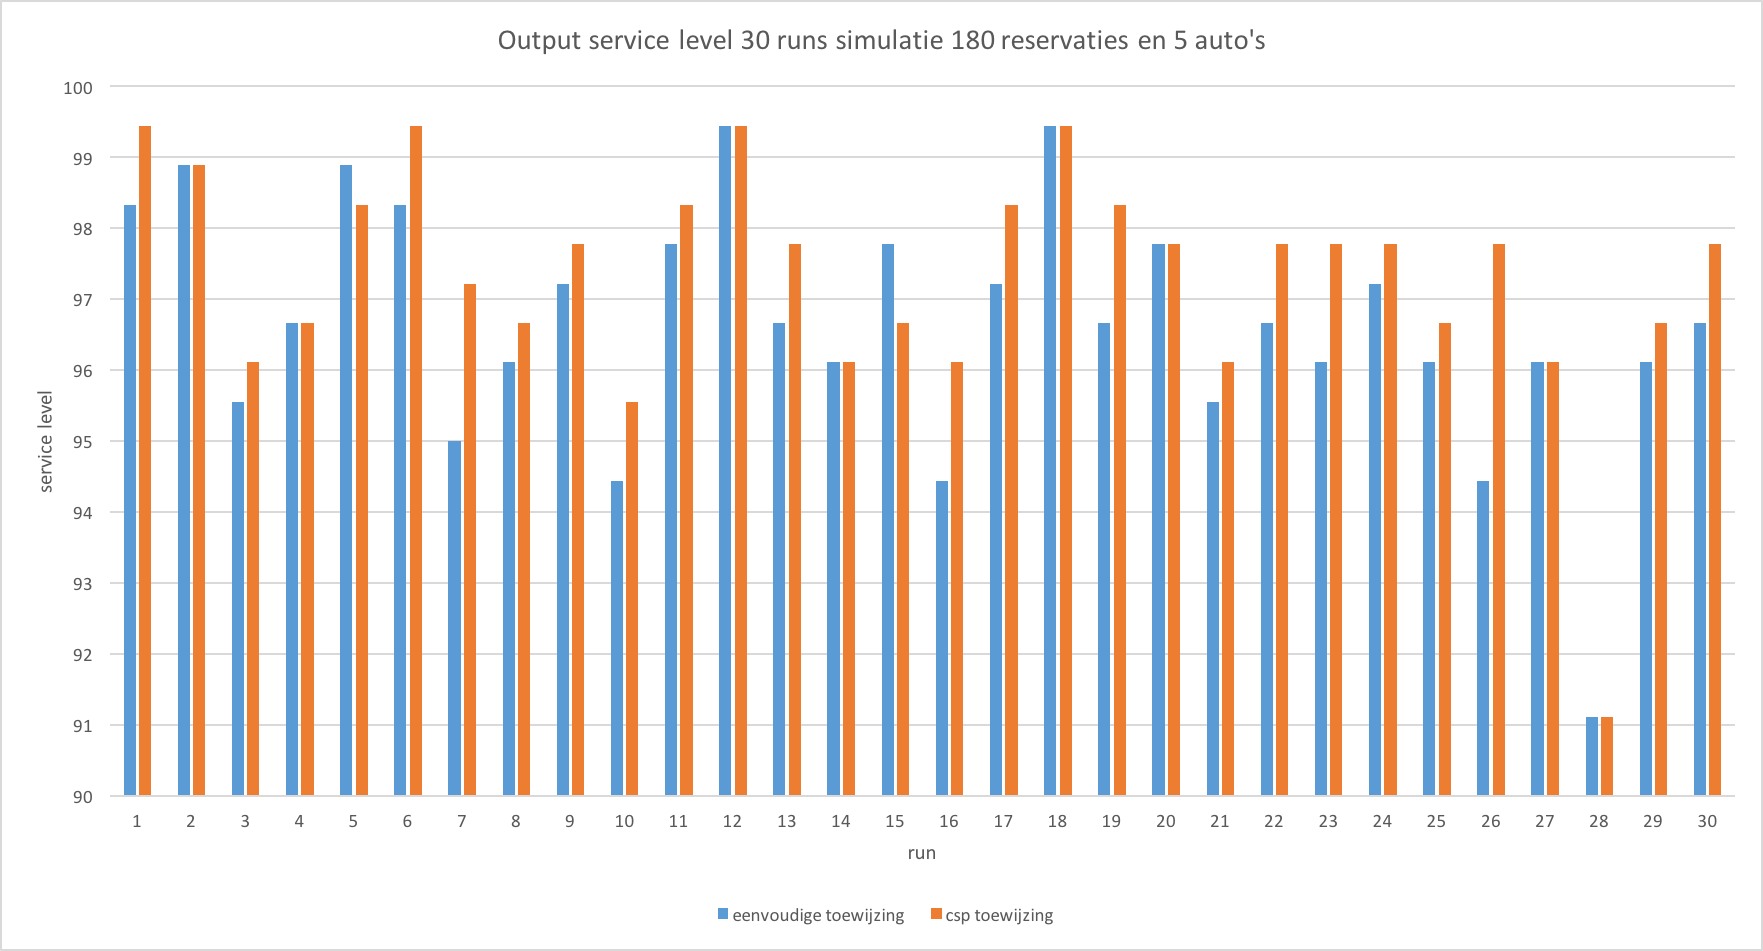
\includegraphics[width=\textwidth]{grafiek-ruwe-output-simulatie.png}
	\caption[Grafiek die de ruwe output data voor het service level van 30 runs van een simulatie weergeeft]{Grafiek die de ruwe output data voor het service level van 30 runs van een simulatie weergeeft}
	\label{grafiek:ruwe-output-simulatie}
\end{figure}

\section{Druktegraad: 9 reservaties/week/auto}
Er werden 2 sets van parameters samengesteld met een druktegraad van 9 reservaties per week per auto. 
De eerste simulatie bestaat uit 108 reservaties verdeeld over 4 weken voor 3 auto's, de tweede bestaat uit 180 reservaties verdeeld over 4 weken voor 5 auto's. 
De gemiddelde resultaten van de simulatie worden weergeven in tabel \ref{tab:resultaten9}
\begin{table}[h]
	\centering
	\begin{tabular}{ | c | p{1.5cm} | p{1.5cm} | p{1.5cm} | p{1.5cm} | p{1.5cm} | p{1.5cm} | p{1.5cm} | p{1.5cm} |}
		\hline
		auto's & $\mu_{ SL}$ eenvoudig & $\sigma^2$ eenvoudig & $\mu_{ t}$ per auto eenvoudig & $\mu_{ SL}$ csp & $\sigma^2$ csp & $\mu_{ t}$ per auto csp & $\mu_{\Delta_{ SL}}$ & $\mu_{\Delta_{ t}}$ \\ \hline
		3 & 94,04 & 2,21 & 97h39m & 94,99 & 2,03 & 100h21m & 0,99 & 8h7m  \\ \hline
		5 & 96,63 & 1,74 & 101h43m & 97,33 & 1,63 & 103h52m & 0,70 & 10h46m \\ \hline
	\end{tabular}
	\caption{Tabel met resultaten van de simulaties met als druktegraad 9 reservaties per week per auto}
	\label{tab:resultaten9}
\end{table}

\section{Druktegraad: 15 reservaties/week/auto}
Er werden 2 sets van parameters samengesteld met een druktegraad van 15 reservaties per week per auto. 
De eerste set bestaat uit 180 reservaties verdeeld over 4 weken voor 3 auto's, de tweede bestaat uit 300 reservaties verdeeld over 4 weken voor 5 auto's. 
De resultaten van de simulatie worden weergeven in tabel \ref{tab:resultaten15}
\begin{table}[h]
	\centering
	\begin{tabular}{ | c | p{1.5cm} | p{1.5cm} | p{1.5cm} | p{1.5cm} | p{1.5cm} | p{1.5cm} | p{1.5cm} | p{1.5cm} |}
		\hline
		auto's & $\mu_{ SL}$ eenvoudig & $\sigma^2$ eenvoudig & $\mu_{ t}$ per auto eenvoudig & $\mu_{ SL}$ csp & $\sigma^2$ csp & $\mu_{ t}$ per auto csp & $\mu_{\Delta_{ SL}}$ & $\mu_{\Delta_{ t}}$ \\ \hline
		3 & 85,54 & 2,40 & 141h09m & 86,98 & 2,45 & 147h08m & 1,44 & 17h56m  \\ \hline
		5 & 90,4 & 1,79 & 150h09m & 91,87 & 1,66 & 156h39m & 1,47 & 32h28m \\ \hline
	\end{tabular}
	\caption{Tabel met resultaten van de simulaties met als druktegraad 15 reservaties per week per auto}
	\label{tab:resultaten15}
\end{table}
\section{Druktegraad: 30 reservaties/week/auto}
Er werden 2 sets van parameters samengesteld met een druktegraad van 30 reservaties per week per auto. 
De eerste set bestaat uit 360 reservaties verdeeld over 4 weken voor 3 auto's, de tweede bestaat uit 600 reservaties verdeeld over 4 weken voor 5 auto's. 
De resultaten van de simulatie worden weergeven in tabel \ref{tab:resultaten30}
\begin{table}[h]
	\centering
	\begin{tabular}{ | c | p{1.5cm} | p{1.5cm} | p{1.5cm} | p{1.5cm} | p{1.5cm} | p{1.5cm} | p{1.5cm} | p{1.5cm} |}
		\hline
		auto's & $\mu_{ SL}$ eenvoudig & $\sigma^2$ eenvoudig & $\mu_{ t}$ per auto eenvoudig & $\mu_{ SL}$ csp & $\sigma^2$ csp & $\mu_{ t}$ per auto csp & $\mu_{\Delta_{ SL}}$ & $\mu_{\Delta_{ t}}$ \\ \hline
		3 & 67,18 & 1,77 & 201h51m & 68,45 & 1,95 & 214h48m & 1,27 & 38h52m  \\ \hline
		5 & 72,44 & 1,83 & 224h09m & 73,93 & 2,61 & 156h39m & 1,48 & 79h50m \\ \hline
	\end{tabular}
	\caption{Tabel met resultaten van de simulaties met als druktegraad 30 reservaties per week per auto}
	\label{tab:resultaten30}
\end{table}

